%% ============================================
%% ================ Preambule =================
%% ============================================
\documentclass[]{scrartcl}
\usepackage[margin = 0.5in]{geometry}

\usepackage[pdftex,unicode, 
colorlinks=true,
linkcolor = blue]{hyperref}	% нумерование страниц, ссылки!!!!ИМЕННО В ТАКОМ ПОРЯДКЕ СО СЛЕДУЮЩИМ ПАКЕТОМ
%\usepackage[warn]{mathtext}				% Поддержка русского текста в формулах
\usepackage[T1, T2A]{fontenc}			% Пакет выбора кодировки и шрифтов
\usepackage[utf8]{inputenc} 			% любая желаемая кодировка
\usepackage[english]{babel}		% поддержка русского языка
\usepackage{wrapfig}					% Плавающие картинки
\usepackage{amssymb, amsmath}			% стилевой пакет для формул
\usepackage{algorithm}
\usepackage{algorithmic} 


\ifpdf
\usepackage{cmap} 				% чтобы работал поиск по PDF
\usepackage[pdftex]{graphicx}
%\usepackage{pgfplotstable}		% Для вставки таблиц.
\pdfcompresslevel=9 			% сжимать PDF
\else
\usepackage{graphicx}
\fi

\graphicspath{{./figures/}}
\usepackage{subcaption}
%% ============================================
%% ================ Info =================
%% ============================================
\title{Название проекта}
\author{\begin{tabular}{c c}
	  	 Добрыня Никитич & Daniil Merkulov \\
		 \texttt{voda@baikal.ru} & \texttt{daniil.merkulov@skoltech.ru} 
		\end{tabular}}
\date{\today}

\begin{document}

\maketitle

\begin{abstract}
Емкое описание предполагаемого проекта в один абзац. Емкое описание предполагаемого проекта в один абзац. Ëмкое описание предполагаемого проекта в один абзац. Это абстракт.
\end{abstract}

\section{Идея}

Обратите внимание на конкретность постановки задачи и её реалистичность. В этом разделе надо вкратце обозначить тему проекта - это повторение/вариация на тему уже готовой статьи, собственная идея, что-нибудь другое. Здесь можно привести немного контекста - например, обуславливающего актуальность проекта.

\subsection{Problem}

В этом разделе необходимо очень конкретно написать решаемую задачу. Понять постановку задачи должен человек с хорошим математическим бэкграундом, но без знаний по узкой теме проекта. В качестве валидации рекомендую дать одному или нескольким знакомым однокурсникам, друзьям и спросить - понятна ли постановка задачи при условии, что они прочитают её так как написано без ваших дополнительных комментариев? 

Напишем и процитируем \cite{kaczmarz1951theorie}:  какую нибудь формулу 
\begin{equation}
x_{k+1} = x_k  + \dfrac{b_{r(i)} - \langle a_{r(i)}, x_k\rangle}{\|a_{r(i)}\|_2^2}a_{r(i)}
\end{equation}

Напишем какой нибудь алгоритм

\begin{algorithm}[h!]
	\caption{Randomized Kaczmarz Algorithm}
	\label{RKalg}
	\begin{algorithmic}[1]
		\STATE Initialize $k \leftarrow 0$
		\FOR {$k=0,1,...$}
		\STATE Select row $j$ from $\{1,2,...m\}$ with probability $\frac{||a_j||^2}{||A||_F^2}$
		\STATE Project $x_{k+1} = x_k + \frac{(b_j - a_j^T x_k)}{||a_j||^2} a_j$
		\STATE Update $k \leftarrow k+1$
		\ENDFOR
	\end{algorithmic}
\end{algorithm}



\section{Outcomes}

Опишите, что конкретно будет выходом Вашего проекта (код, теорема, численные эксперименты, телеграм бот, веб сайт, приложение, рассказ).

\begin{figure}[h!]
	\center{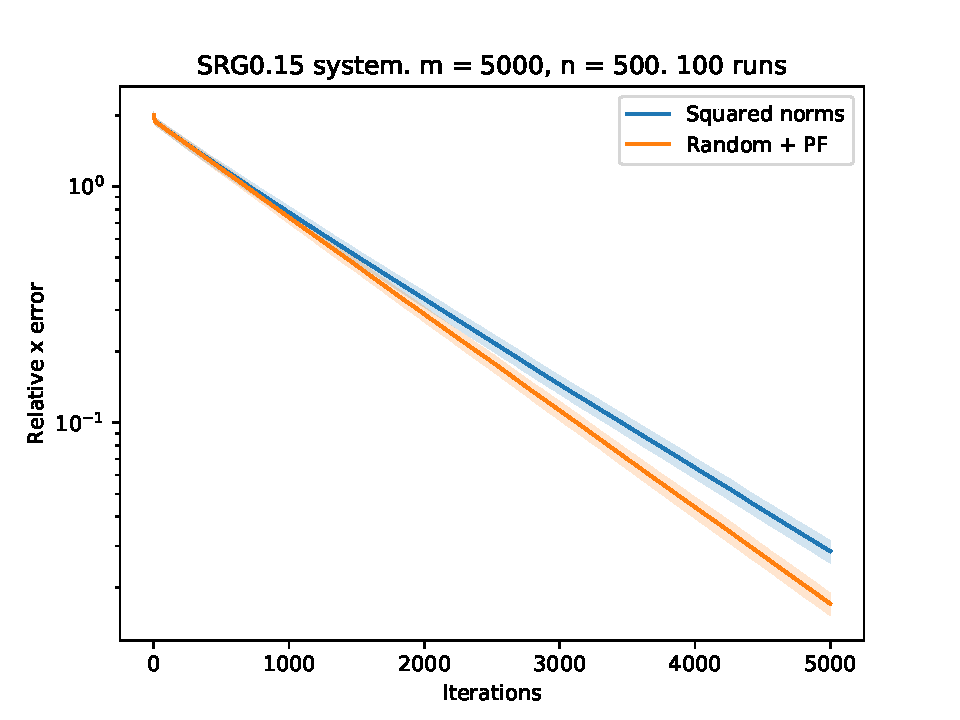
\includegraphics[width=0.3\linewidth]{test.pdf}}
	\caption{Картинка, иллюстрирующая идею / выход проекта}
\end{figure}


\section{Литературный обзор}
Краткий обзор релевантных источников по теме, со ссылками на них - минимальное число источников - 7.


В работе \cite{strohmer2009randomized} исследовалось то-то, и даже есть формула:
\begin{equation}
\mathbb{E} \|x_k - x\|_2^2 \leq \left(1 - \kappa (A) ^{-2}\right)^k \|x_0 - x\|_2^2
\end{equation}


А вот в этих работах другой очень интересный взгляд \cite{gower2015randomized}, \cite{dai2014randomized} 

\section{Метрики качества}
Приведите формальные и измеряемые показатели, по которым можно оценивать Ваше решение\ проект - это могут быть конкретные метрики качества алгоритмов, соц. опрос, логическое доказательство и т.д. Наша задача в этом разделе - суметь легко ответить на вопрос работает ли данная идея в конкретных задачах или нет (отрицательный результат тоже результат)

\section{Примерный план}
\begin{itemize}
	\item Сначала это к такому то сроку
	\item Потом вот это
	\item И это - программа минимум
	\item А вот это  - если успею программу минимум
\end{itemize}

\section{Отчёт о фазе прототипирования}
Мы попробовали провести эксперименты с существующим кодом - у нас получились такие результаты, попробовали немного изменить постановку, всё сломалось. Вот скриншоты. Вот потребление памяти. Вот это место, в котором неравенство не верно.

\bibliographystyle{unsrt}
\bibliography{biblio}

\end{document}
